\documentclass{exam}
\usepackage{../../commonheader}
\usepackage{graphicx}
\usepackage{color}

%%% CHANGE THESE %%%%%%%%%%%%%%%%%%%%%%%%%%%%%%%%%%%%%%%%%%%%%%%%%%%%%%%%%%%%%%
\discnumber{3}
\title{\textsc{Midterm 1 Review}}
\date{February 15, 2017}
%%%%%%%%%%%%%%%%%%%%%%%%%%%%%%%%%%%%%%%%%%%%%%%%%%%%%%%%%%%%%%%%%%%%%%%%%%%%%%%

\begin{document}
\maketitle
\rule{\textwidth}{0.15em}
\fontsize{12}{15}\selectfont

%%% INCLUDE TOPICS HERE %%%%%%%%%%%%%%%%%%%%%%%%%%%%%%%%%%%%%%%%%%%%%%%%%%%%%%%


%%% Question %%%

\section{Control}
\begin{questions}

\item Fill in the blanks of \texttt{sum\_k\_digits}. \texttt{sum\_k\_digits} takes in two integers, \texttt{n} and \texttt{k} and sums the rightmost \texttt{k} digits of \texttt{n}. If \texttt{k} is greater than \texttt{n}, sum up all of the digits. See the doctests for more details:
\newline
\begin{lstlisting}
def sum_k_digits(n, k):
	""" Returns the sum of the rightmost k digits of n. Assume n has >= k digits.
	     >>> sum_k_digits(11111, 3)
	     3
	     >>> sum_k_digits(12345, 2)
	     9
	"""
	total = ______________________________
	
	while _______________________________:
	
		total = ______________________________
		
		n = ________________________________
		
		k = ________________________________
		
	return ________________________________


\end{lstlisting}
\begin{solution}
\begin{lstlisting}
def sum_k_digits(n, k):
	""" Returns the sum of the rightmost k digits of n. Assume n has >= k digits.
	     >>> sum_k_digits(11111, 3)
	     3
	     >>> sum_k_digits(12345, 2)
	     9
	"""
	total = 0
	while k > 0:
		total = total + (n % 10)
		n = n // 10
		k = k - 1
	return total

\end{lstlisting}
\end{solution}

\item \textbf{Extra: } How would you solve it recursively?
\begin{solution}
\begin{lstlisting}
def sum_k_digits(n, k):
	""" Returns the sum of the rightmost k digits of n. Assume n has >= k digits.
	     >>> sum_k_digits(11111, 3)
	     3
	     >>> sum_k_digits(12345, 2)
	     9
	"""
	if k == 0:
	   return 0
	return n % 10 + sum_k_digits(n//10, k-1)

\end{lstlisting}
\end{solution}
\end{questions}
\clearpage

\section{Environment Diagrams}
\begin{questions}
\item Fill in the environment diagram that results from executing the code below until the entire program
is finished or an error occurs. You may not need to use all of the spaces or frames.
A complete answer will:
\begin{itemize}
\item  Add all missing names and parent annotations to all local frames.
\item  Add all missing values created or referenced during execution.
\item Show the return value for each local frame. 
\end{itemize}
\vspace{1 cm}
\begin{lstlisting}
sam = "ss"

def josiah(leo):
    sam = "it"
    def josh(cj):
        donna = cj(sam, "sag") 
        return donna + leo
    return josh

president = josiah("tarius")
password = president(lambda josh, toby: toby + josh)
\end{lstlisting}


\begin{solution}
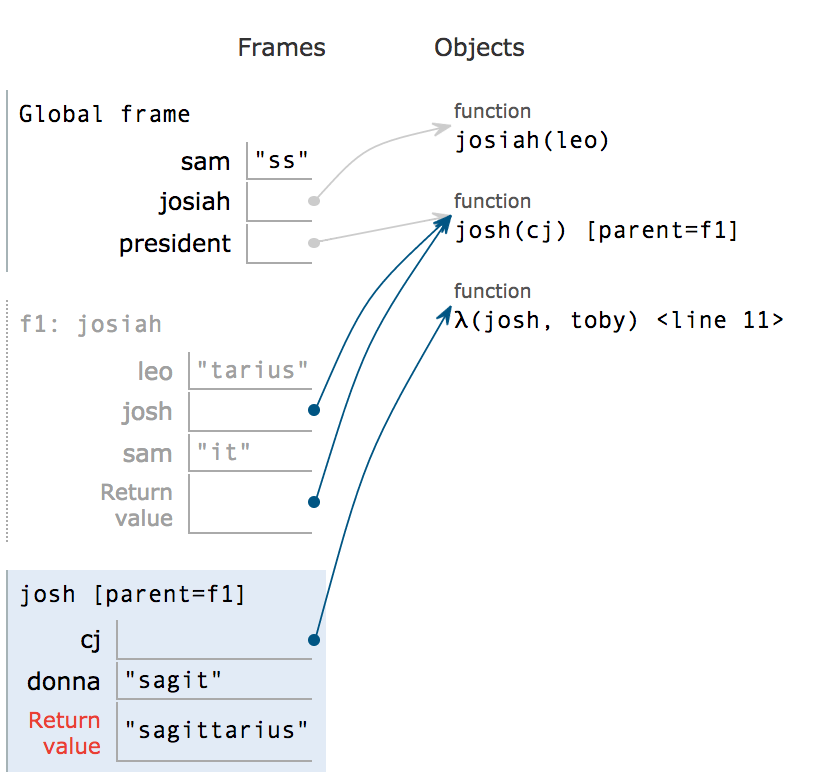
\includegraphics[width=7cm]{env1}
\end{solution}

\clearpage

\item Fill in the environment diagram that results from executing the code below until the entire program
is finished or an error occurs. You may not need to use all of the spaces or frames.
A complete answer will:
\begin{itemize}
\item  Add all missing names and parent annotations to all local frames.
\item  Add all missing values created or referenced during execution.
\item Show the return value for each local frame. 
\end{itemize}
\vspace{1 cm}
\begin{lstlisting}
def never(the, less):
    if the < less:
        return 'never'
    elif not less:
        print('always')
    if less == -3:
        return never(less, the)
    return never(less, less - the)

never(3, 0)
\end{lstlisting}


\begin{solution}
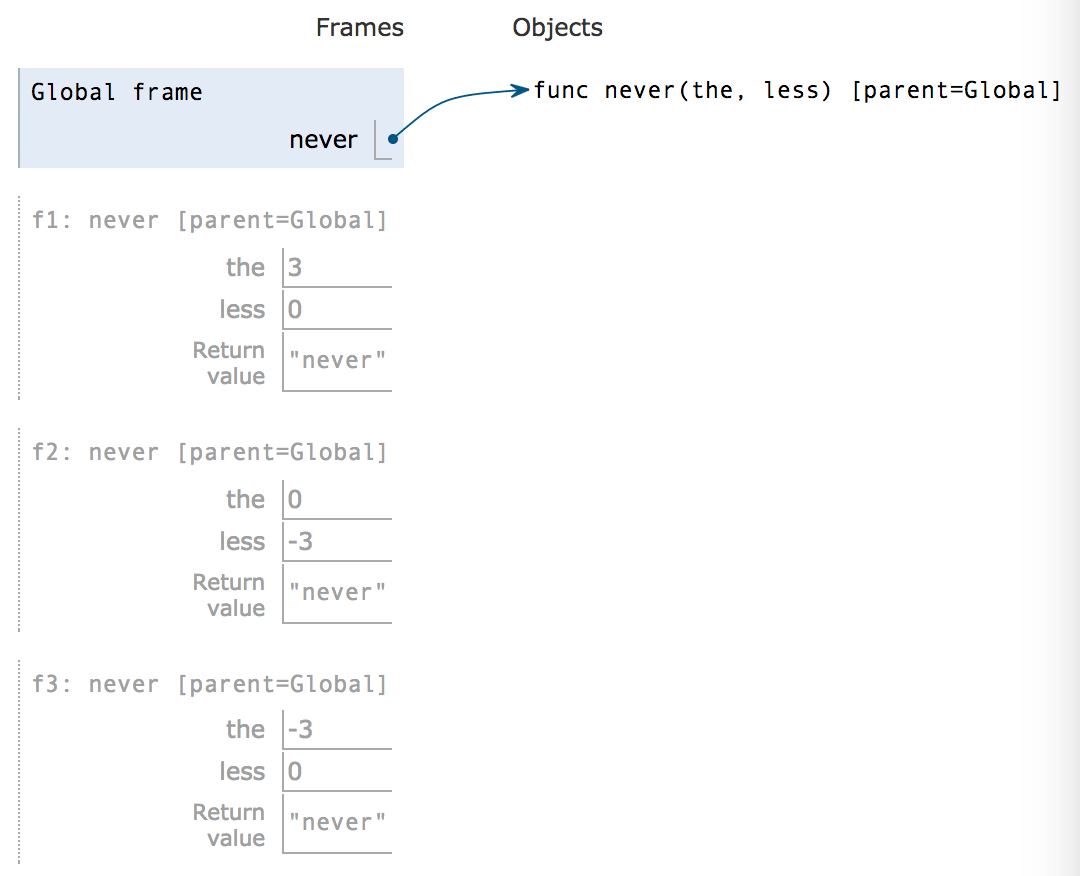
\includegraphics[width=10cm]{env2}
\end{solution}
\end{questions}

\clearpage

\section{What Would Python Display}
\begin{questions}
\item For each of the expressions in the table below, write the output displayed by the interactive Python interpreter when the expression is evaluated. The output may have multiple lines. If an error occurs, write “Error”.
Assume that you have started \texttt{python3} and executed the following statements:

\begin{lstlisting}
def pup(bark):
   woof = 10;
   def yip(yap):
      if bark % yap == 0:
         return woof * 3
      return yap + woof
   return yip
def spot(dog):
   per = 39
   if dog > 5:
      print("pup")
   if dog > 10:
      return pup(per)
def cloud(grr):
   print(grr * 3)
woof = 9
\end{lstlisting}
\begin{center}
    \begin{tabular}{|m{8cm}|m{6cm}|}
\hline
\textbf{Expression} & \textbf{Interactive Output} \\
\hline
\lstinline$py = woof % 3$ &  \\ & \\
\hline
\lstinline$pet = spot(13)$ & \\ & \\
\hline
\lstinline$print(cloud(woof + 6))$ & \\ & \\ & \\
\hline
\lstinline$pet(py)$ & \\ & \\
\hline
\lstinline$pet(woof)$& \\ & \\
\hline
\lstinline$pup(py)$ & \\ & \\
\hline
\lstinline$pet(3)$ & \\ & \\
\hline
\end{tabular}
\end{center}

\begin{solution}
\begin{center}
    \begin{tabular}{|m{8cm}|m{6cm}|}
\hline
\textbf{Expression} & \textbf{Interactive Output} \\
\hline
\lstinline$py = woof % 3$ &  \\ & \\
\hline
\lstinline$pet = spot(13)$ & \color{red}\texttt{pup} \\ & \\
\hline
\lstinline$print(cloud(woof + 6))$ & \color{red}\texttt{45}\\ & \color{red}\texttt{None}\\ & \\
\hline
\lstinline$pet(py)$ & \color{red}\texttt{Error}\\ & \\
\hline
\lstinline$pet(woof)$& \color{red}\texttt{19}\\ & \\
\hline
\lstinline$pup(py)$ & \color{red}\texttt{Function}\\ & \\
\hline
\lstinline$pet(3)$ & \color{red}\texttt{30}\\ & \\
\hline
\end{tabular}
\end{center}
\end{solution}

\clearpage

\item \textbf{Extra:}
For each of the expressions in the table below, write the output displayed by the interactive Python interpreter when the expression is evaluated. The output may have multiple lines. If an error occurs, write “Error”.
Assume that you have started \texttt{python3} and executed the following statements:

\begin{lstlisting}
def dell(ta):
   lamduh = [3, 1, 4, 1, 5, 9]
   pie = lamduh
   def eye(ota):
      return lambda pie, kye: pie[:-2] + kye[ota[0]::-1]
   lamduh = lamduh + ta
   print(pie)
   return eye

def bay(ta):
   row = [ca - 9 for ca in ta]
   print(row, ta)
   return dell
 
\end{lstlisting}
\vspace{1 cm}
\begin{center}
    \begin{tabular}{|m{8cm}|m{6cm}|}
\hline
\textbf{Expression} & \textbf{Interactive Output} \\
\hline
\lstinline$fie = [2, 17, 20, 17]$ &  \\ & \\
\hline
\lstinline$nul = [0, -1, -50]$ & \\ & \\
\hline
\lstinline$gam = bay(fie)$ & \\ & \\ & \\
\hline
\lstinline$tao = gam(nul)$ & \\ & \\
\hline
\lstinline$print(tao([1, 5, 7])(fie, nul))$& \\ & \\
\hline
\end{tabular}
\end{center}
\clearpage
\begin{solution}
\begin{center}
    \begin{tabular}{|m{8cm}|m{6cm}|}
\hline
\textbf{Expression} & \textbf{Interactive Output} \\
\hline
\lstinline$fie = [2, 17, 20, 17]$ &  \\ & \\
\hline
\lstinline$nul = [0, -1, -50]$ & \\ & \\
\hline
\lstinline$gam = bay(fie)$ & \color{red}\texttt{[-7, 8, 11, 8] [2, 17, 20, 17]
}\\ & \\ & \\
\hline
\lstinline$tao = gam(nul)$ & \color{red}\texttt{[3, 1, 4, 1, 5, 9]}\\ & \\
\hline
\lstinline$print(tao([1, 5, 7])(fie, nul))$& \color{red}\texttt{[2, 17, -1, 0]}\\ & \\
\hline
\end{tabular}
\end{center}
\end{solution}
\end{questions}

\section{Higher Order Functions}
\begin{questions}
\item Fill in the blanks so that the doctest passes.

\begin{lstlisting}
def repeated(f, n):
   """
   >>> repeated(lambda x: x*x, 2)(2)
   16
   """
    g = lambda x: x
    
    while ______________________________:
        
        g = ______________________________
        
        ______________________________
    
    return g
\end{lstlisting}

\begin{solution}
\begin{lstlisting}
    g = lambda x: x
    while n > 0:
        g = lambda x: f(g(x))
        n -= 1
    return g
\end{lstlisting}
\end{solution}
\end{questions}

\section{Recursion}
\begin{questions}
\item Fill in the blanks to \texttt{replace}, so that it returns a number identical to n, but where every digit old is replaced with digit new.
\begin{lstlisting}
def replace(n, old, new): 
   if ____________________________________________:
        return 0        
    last = ____________________________________________
    
    rest = ____________________________________________   
     
    if last == old:
    
         _______________________________________________________
    else:    
        _______________________________________________________
\end{lstlisting}

\begin{solution}
\begin{lstlisting}
   if n == -:
        return 0
    last = n % 10
    rest = n //10
    if last == old:
         return replace(rest, old, new) * 10 + new
    else:
        return replace(rest, old, new) * 10 + last

\end{lstlisting}
\end{solution}

\item Write a function that takes as input a number \texttt{n} and a list of numbers \texttt{lst} and returns \texttt{True} if we can find a subsequence of \texttt{lst} that sums up to \texttt{n}
\begin{lstlisting}
def addup(n, old, new): 
    """ 
    >>> addup(10, [1, 2, 3, 4, 5])
    True
    >>> addup(8, [1, 2, 3, 4, 5])
    True
    >>> addup(-1, [1, 2, 3, 4, 5])
    False
    >>> addup(100, [1, 2, 3, 4, 5])
    False
    """
    if __________________________________________:
    
        return True
        
    if lst == []:
    
        ____________________________________________________
        
    else:
    
        first, rest = ____________________, ____________________
        
        return __________________________________________
\end{lstlisting}

\begin{solution}
\begin{lstlisting}
    if n == 0:
        return True
    if lst == []:
         return False  
    else:
        first, rest = lst[0], lst[1:]
        return addup(n - first, rest) or addupt(n, rest)

\end{lstlisting}
\end{solution}
\end{questions}

\clearpage 

\section{Linked Lists and Trees}
Here are the constructors and selectors of \texttt{link} and \texttt{tree}:
\begin{center}
    \begin{tabular}{|m{8cm}|m{8cm}|}
\hline
\begin{lstlisting}
# Linked List definition
empty = 'empty'

def link(first, rest=empty):
    return [first, rest]

def first(s):
    return s[0] 
    
def rest(s):
    return s[1]
    \end{lstlisting}
    
    
    
    & \begin{lstlisting}
# Tree definition
def tree(label, branches=[]):
    return [label] + list(branches)

def label(t):
    return t[0]

def branches(t): 
    return t[1:]
    \end{lstlisting} \\

\hline
\end{tabular}
\end{center}


\begin{questions}
\item Write a function that takes in a linked list, lnk, and returns a linked list that is the reverse of lnk. That is, the first element of the returned list is the last element of lnk, the second element is the second to last element of lnk, and so on.

\begin{lstlisting}
def reverse(lnk):
    >>> reverse(link(1, empty)))
    link(1, empty)
    >>> reverse(link(2, link (4, empty))
    link(4, link(2, empty))
    def reverse(lnk):
    
        reversed =  ________________________________________
        
        while ________________________________:
        
            reversed = _______________________________________
            
            lnk = _____________________________
            
        return _____________________________________________

\end{lstlisting}

\begin{solution}
\begin{lstlisting}
        reversed =  empty
        while lnk != empty:        
            reversed = link(first(lnk), reversed)            
            lnk = rest(lnk)            
        return reversed
\end{lstlisting}
\end{solution}

\clearpage

\item Write a function that returns true only if there exists a path from root to leaf that contains at least n instances of elem in a tree t.
\begin{lstlisting}
def contains_n(elem, n, t):
    >>> t1 = tree(1, [tree(1,tree(2)])
    >>> contains(1, 2, t1)
    True
    >>> contains(2, 2, t1)
    False
    >>> contains(2, 1, t1)
    True
    >>> t2 = tree(1, [tree(2), tree(1, [tree(1), tree(2)])
    >>> contains(1, 3, t1)
    True
    >>> contains(2, 2, t1) # Not on a path
    False
    if n == 0:
    
        return True
        
    elif n == 1 and __________________________________:
    
        return True
        
    elif __________________________________:
    
        return __________________________________
        
    elif label(t) == elem:
    
        return ______________________________________________
        
    else:
    
        return __________________________________
        
\end{lstlisting}

\begin{solution}
\begin{lstlisting}
    if n == 0:
        return True
    elif n == 1 and is_leaf(t) and label(t) == elem:
        return True
    elif is_leaf(t):
        return False
    elif label(t) == elem:
        return True in [contains_n(elem, n - 1, b) for b in     
          branches(t)]
    else:
        return True in [contains_n(elem, n, b) for b in 
          branches(t)]
\end{lstlisting}
\end{solution}
\end{questions}
%%%%%%%%%%%%%%%%%%%%%%%%%%%%%%%%%%%%%%%%%%%%%%%%%%%%%%%%%%%%%%%%%%%%%%%%%%%%%%%

\end{document}
